%----------------------------------------------------------------------------------------
%	PACKAGES AND OTHER DOCUMENT CONFIGURATIONS
%----------------------------------------------------------------------------------------

\documentclass{article}

\usepackage{fancyhdr} % Required for custom headers
\usepackage{lastpage} % Required to determine the last page for the footer
\usepackage{extramarks} % Required for headers and footers
\usepackage[usenames,dvipsnames]{color} % Required for custom colors
\usepackage{graphicx} % Required to insert images
\usepackage{listings} % Required for insertion of code
\usepackage{courier} % Required for the courier font
\usepackage{lipsum} % Used for inserting dummy 'Lorem ipsum' text into the template
\usepackage{color}
\usepackage{amsmath}
\usepackage{float}
\usepackage[titletoc]{appendix}
\usepackage{caption}
\usepackage{framed,color}

% Margins
\topmargin=-0.45in
\evensidemargin=0in
\oddsidemargin=0in
\textwidth=6.5in
\textheight=9.0in
\headsep=0.25in

\linespread{1.1} % Line spacing

% Set up the header and footer
\pagestyle{fancy}
%\lhead{\hmwkAuthorName} % Top left header
\lhead{} % Top left header
\chead{\hmwkTitle} % Top center head
\rhead{\firstxmark} % Top right header
\lfoot{\lastxmark} % Bottom left footer
\cfoot{} % Bottom center footer
\rfoot{Page\ \thepage\ of\ \protect\pageref{LastPage}} % Bottom right footer
\renewcommand\headrulewidth{0.4pt} % Size of the header rule
\renewcommand\footrulewidth{0.4pt} % Size of the footer rule

\setlength\parindent{0pt} % Removes all indentation from paragraphs

%----------------------------------------------------------------------------------------
%	CODE INCLUSION CONFIGURATION
%----------------------------------------------------------------------------------------
\definecolor{dkgreen}{rgb}{0,0.6,0}
\definecolor{gray}{rgb}{0.5,0.5,0.5}
\definecolor{mauve}{rgb}{0.58,0,0.82}
\definecolor{shadecolor}{rgb}{0.9,0.9,0.9}

\lstset{frame=tb,
  language=Java,
  aboveskip=3mm,
  belowskip=3mm,
  showstringspaces=false,
  columns=flexible,
  basicstyle={\small\ttfamily},
  numbers=none,
  numberstyle=\tiny\color{gray},
  keywordstyle=\color{blue},
  commentstyle=\color{dkgreen},
  stringstyle=\color{mauve},
  breaklines=true,
  breakatwhitespace=true
  tabsize=3
}

%----------------------------------------------------------------------------------------
%	DOCUMENT STRUCTURE COMMANDS
%	Skip this unless you know what you're doing
%----------------------------------------------------------------------------------------

% Header and footer for when a page split occurs within a problem environment
\newcommand{\enterProblemHeader}[1]{
\nobreak\extramarks{}{}\nobreak
\nobreak\extramarks{}{}\nobreak
}

% Header and footer for when a page split occurs between problem environments
\newcommand{\exitProblemHeader}[1]{
\nobreak\extramarks{}{}\nobreak
}

\setcounter{secnumdepth}{0} % Removes default section numbers
\newcounter{homeworkProblemCounter} % Creates a counter to keep track of the number of problems

\newcommand{\homeworkProblemName}{}
\newenvironment{homeworkProblem}[1][Problem \arabic{homeworkProblemCounter}]{ % Makes a new environment called homeworkProblem which takes 1 argument (custom name) but the default is "Problem #"
\stepcounter{homeworkProblemCounter} % Increase counter for number of problems
\renewcommand{\homeworkProblemName}{\arabic{homeworkProblemCounter}. #1} % Assign \homeworkProblemName the name of the problem
\section{\homeworkProblemName} % Make a section in the document with the custom problem count
\enterProblemHeader{\homeworkProblemName} % Header and footer within the environment
}{
\exitProblemHeader{\homeworkProblemName} % Header and footer after the environment
}

\newcommand{\problemAnswer}[1]{ % Defines the problem answer command with the content as the only argument
\noindent\begin{minipage}{1.00\columnwidth}#1\end{minipage} % Makes the box around the problem answer and puts the content inside
}

%----------------------------------------------------------------------------------------
%	NAME AND CLASS SECTION
%----------------------------------------------------------------------------------------

\newcommand{\hmwkTitle}{Longest Sequence Algorithms} % Assignment title
\newcommand{\hmwkSubTitle}{} % Assignment subtitle
\newcommand{\hmwkDueDate}{Thursday,\ December\ 5,\ 2013} % Due date
\newcommand{\hmwkClass}{CSCI-665 Foundations of Algorithms} % Course/class
\newcommand{\hmwkAuthorName}{Daniel Cappuccio \& Jason A. Smith} % Your name

%----------------------------------------------------------------------------------------
%	USEFUL COMMANDS
%----------------------------------------------------------------------------------------


\newcommand{\BigO}[1]{\ensuremath{\operatorname{O}\bigl(#1\bigr)}}

%----------------------------------------------------------------------------------------
%	TITLE PAGE
%----------------------------------------------------------------------------------------

\title{
\vspace{2in}
\textmd{\textbf{\hmwkClass}}\\
\textmd{\textbf{\hmwkTitle}}\\
\vspace{0.1in}\large{\textit{\hmwkSubTitle}}\\
\normalsize\vspace{0.1in}\small{\hmwkDueDate}
\vspace{3in}
}

\author{\textbf{\hmwkAuthorName}}
\date{} % Insert date here if you want it to appear below your name

%----------------------------------------------------------------------------------------

\begin{document}

\maketitle

\newpage

%----------------------------------------------------------------------------------------

\begin{homeworkProblem}[Section 01]

A...
\\\\
The...

\end{homeworkProblem}

%----------------------------------------------------------------------------------------

\begin{homeworkProblem}[Section 02]

The formula for query time takes the form \begin{equation}
\label{first}
Q = 7.25 + 52.78 \log _{10} N
\end{equation} where $Q$ is...

\end{homeworkProblem}

%----------------------------------------------------------------------------------------

\begin{homeworkProblem}[Section 03]

The \texttt{ChordQueryTime} class is...
\\\\
Usage statement:

\begin{snugshade}
\verb,$ java ChordQueryTime <log N_L> <log N_U> <log N_D> \, \\
\verb,                      <max_routers> <max_query_length> <T> <seed>, 
\end{snugshade}

\end{homeworkProblem}

%----------------------------------------------------------------------------------------

\begin{homeworkProblem}[Section 04]

See \textbf{Appendix A} for complete source code.

\end{homeworkProblem}

%----------------------------------------------------------------------------------------

\begin{homeworkProblem}[Section 05]

\begin{snugshade}
\verb,$ java ChordQueryTime 2 4 0.1 0 0 1000 1234,\\
\verb,      Query time,, \verb,Q,\\
\verb,N     Mean Stddev,\\
\verb,100   3.34 2.51,\\
\verb,126   3.99 3.01,\\
\end{snugshade}

\vspace{-15pt}
\begin{figure}[H]
\caption{}
\end{figure}
\vspace{-20pt}

\end{homeworkProblem}

%----------------------------------------------------------------------------------------

\begin{homeworkProblem}[Section 06]

\begin{figure}[H]
\center{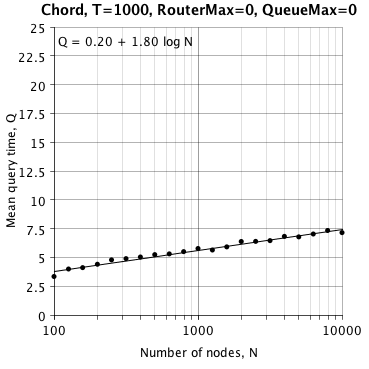
\includegraphics[width=0.5\textwidth] {chord_1000_0_0}}
\caption{}
\end{figure}

\end{homeworkProblem}

%----------------------------------------------------------------------------------------

\newpage
\begin{homeworkProblem}[References]

[1] I. Stoica, R. Morris, D. Liben-Nowell, D. R. Karger, F. Kaashoek, F. Dabek, and H. Balakrishnan. Chord: a scalable peer-to-peer lookup protocol for internet applications. IEEE/ACM Transactions on Networking, 11(1):17-32, February 2003.\\

[2] Computer Science Course Library, Prof. Alan Kaminsky, Rochester Institute of Technology -- Department of Computer Science; http://www.cs.rit.edu/\verb,~,ark/cscl.shtml\\

\end{homeworkProblem}

%----------------------------------------------------------------------------------------

\newpage
\appendix
\section{\\Appendix A} \label{App:AppendixA}

%----------------------------------------------------------------------------------------

\end{document}